\subsection{Failure-set distance as an error signal}
\label{app:signal}
Figure~\ref{fig:signal} reports discrimination of incorrect B0 predictions. A larger AUROC is better; signs are chosen so that low B0 confidence and small failure-set distance indicate an error. The random-set curve here uses the diagnostic random subset in \texttt{vrf\_signal.csv}; the accuracy control V0 averages 20 random-set draws in \texttt{vrf\_summary.csv}.
\begin{figure}[htbp]
\centering
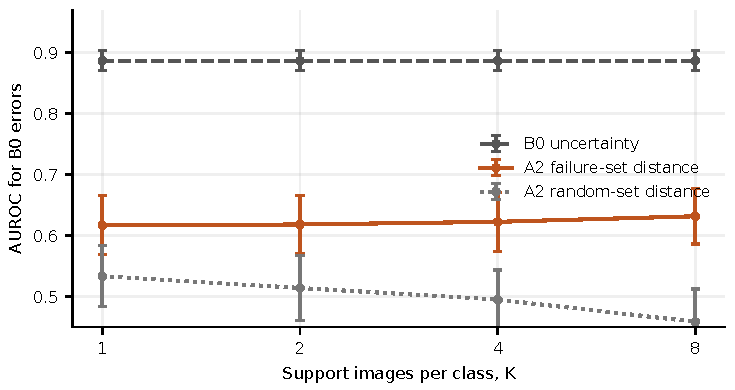
\includegraphics[width=0.78\linewidth]{report/figures/signal.pdf}
\caption{AUROC for detecting B0 errors, averaged equally over domains and seeds. Failure-set distance provides some signal, but less than B0 uncertainty in all plotted settings. Error bars are one sample standard deviation over the 20 domain--seed conditions at each $K$.}
\label{fig:signal}
\end{figure}
